\subsection{Standard Model W$\gamma$ Production}

A $W$ boson in the proton-proton collisions can be produced in the processes $q {\bar{q'}} \rightarrow W$ where $q$ and $\bar{q'}$ are a quark and an antiquark which have a total charge of $+1$ if producing a $W^+$ boson or of $-1$ if producing a $W^-$ boson. The processes $u\bar{d}\rightarrow W^+$ and $d\bar{u}\rightarrow W^-$ are the most likely to occur because $u$ and $d$ are valence quarks in a proton. Antiquarks $\bar{d}$ and $\bar{u}$ come from sea $q\bar{q}$ pairs of the other proton.\\

Decay modes of a $W$ boson include $W^\pm \rightarrow l^\pm \nu_l ({\bar{\nu_l}})$ where $l^\pm=e^\pm$, $\mu^\pm$ or $\tau^\pm$ with branching fractions of ~11\% per a leptonic channel \cite{ref_PDG}. The rest 67\% stands for various $W\rightarrow q\bar{q'}$ decays. In this dissertation we only consider $W^\pm \rightarrow \mu^\pm \nu_\mu ({\bar{\nu_\mu}})$ and $W^\pm \rightarrow e^\pm \nu_e ({\bar{\nu_e}})$ as the cleanest channels.\\

Mass of a $W$ boson $M_W=80~GeV$ is much larger than masses of its decay products: $M_\mu=105~MeV$, $M_e=0.5~MeV$, $M_\nu<2~eV$. Therefore, almost all mass of a $W$ boson converts to the kinetic energy of a muon(electron) and a neutrino.\\

A photon can be emitted from any charged particle of the process: a quark, an antiquark, a charged lepton or a $W$ boson (Fig. \ref{fig:feynmWg_LO_NLO}, top). A quark and an antiquark are initial state particles and, therefore, if one of them radiates a photon, we call such process the Initial State Radiation (ISR). A muon or an electron is a final state particle and if it radiates a photon, we call such process the Final State Radiation (FSR). Finally, a $W$ boson is a gauge boson and if it radiates a photon, the process has a vertex with three gauge bosons: $WW\gamma$, and we call such process the Triple Gauge coupling (TGC).\\

\begin{figure}[htb]
  \begin{center}
    {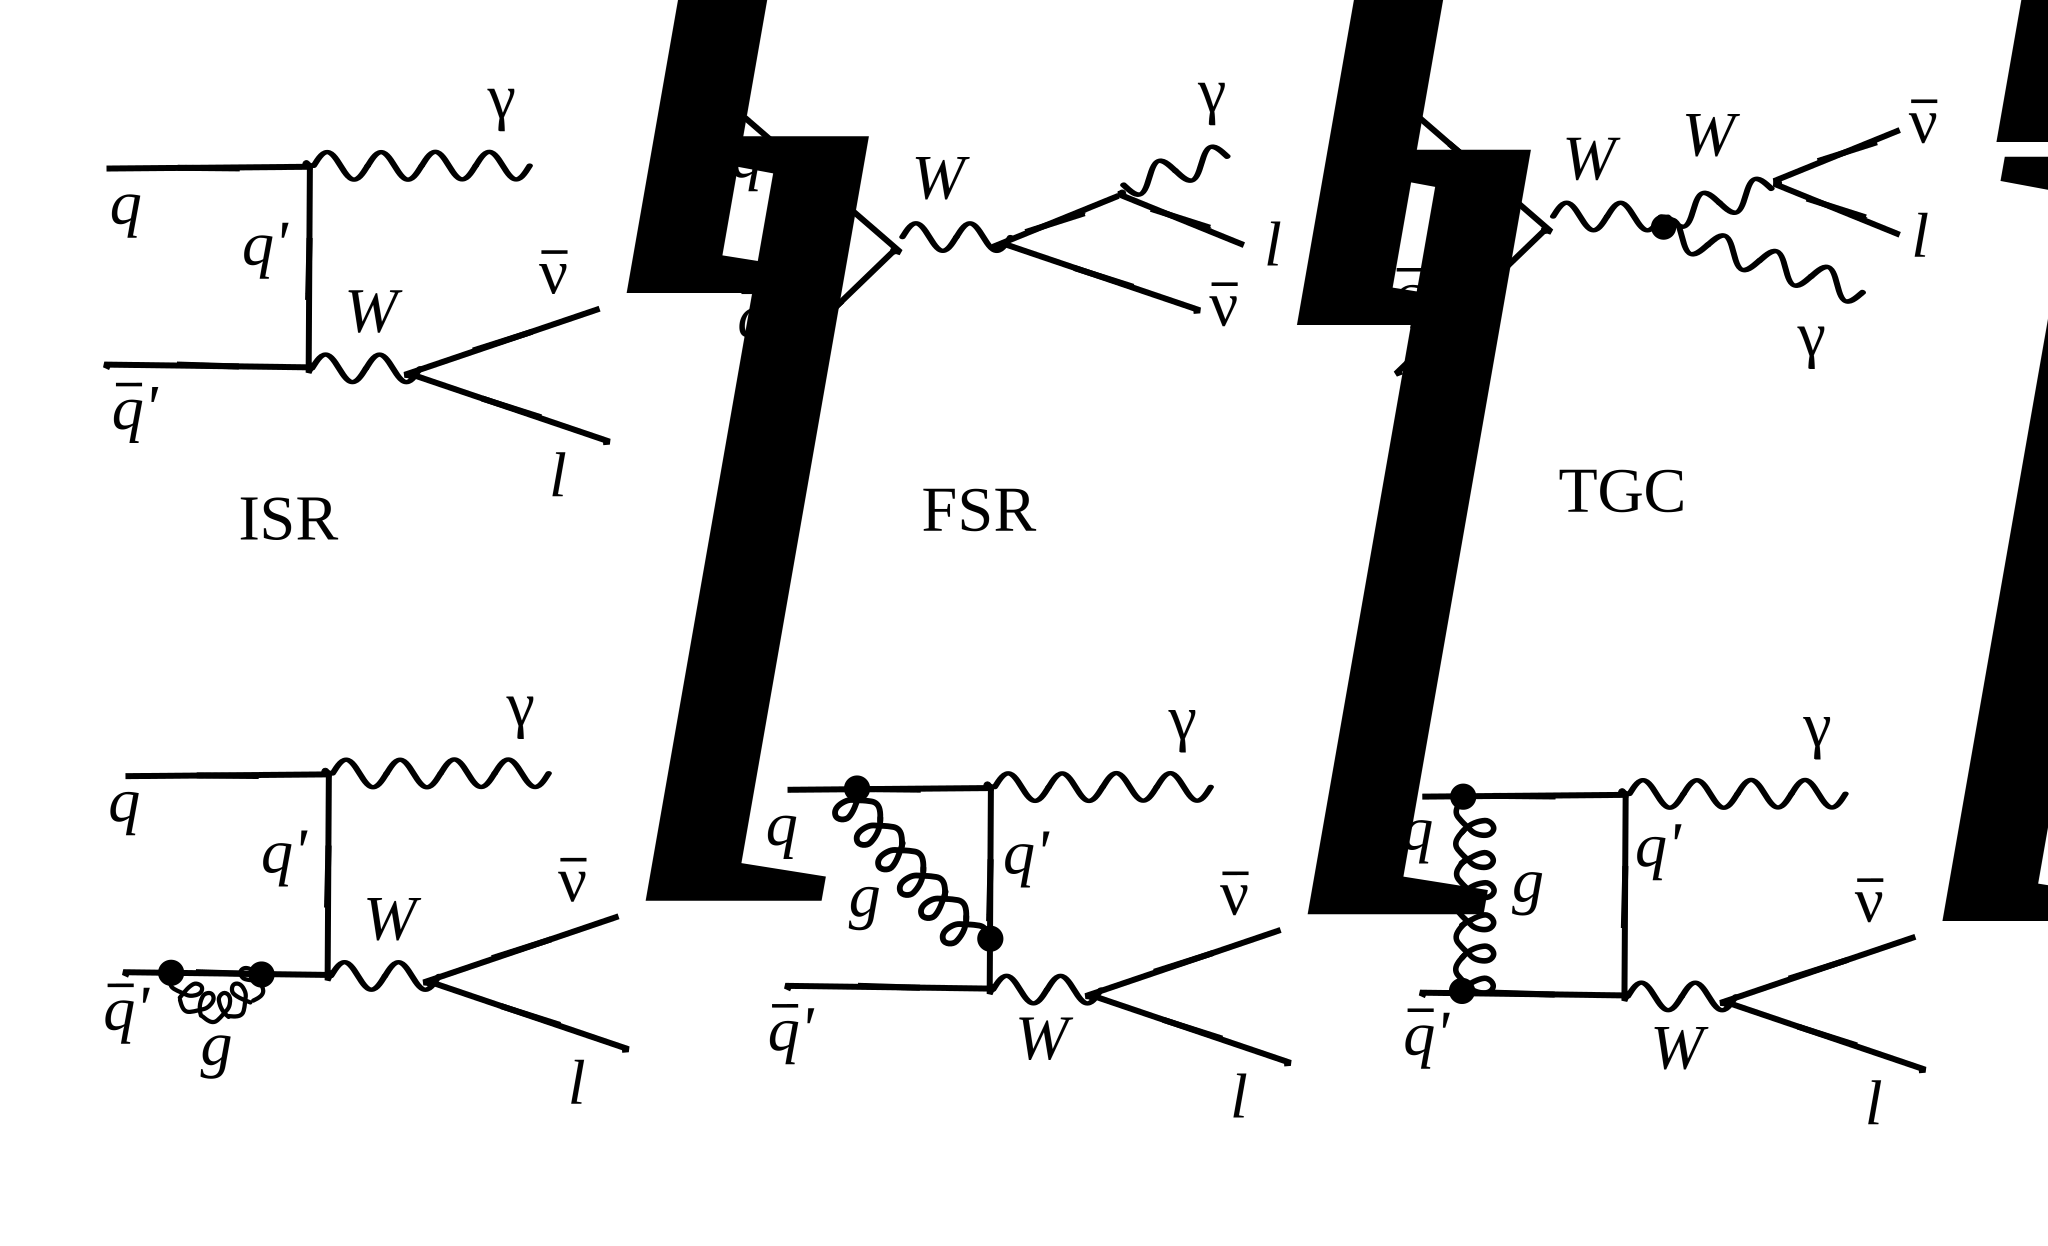
\includegraphics[width=0.90\textwidth]{../figs/WgAbout/feynmWg_LO_NLO.png}}
    \caption{Feynman diagrams of W$\gamma$ production}
    \label{fig:feynmWg_LO_NLO}
  \end{center}
\end{figure}

%Explain Feynman diagrams
%Need Griffiths

%Give a definitions of the total and differential cross section of the Standard Model processes
%Explain LO/NLO/NNLO thing
%Need Griffiths and/or PDG

\begin{figure}[htb]
  \begin{center}
    {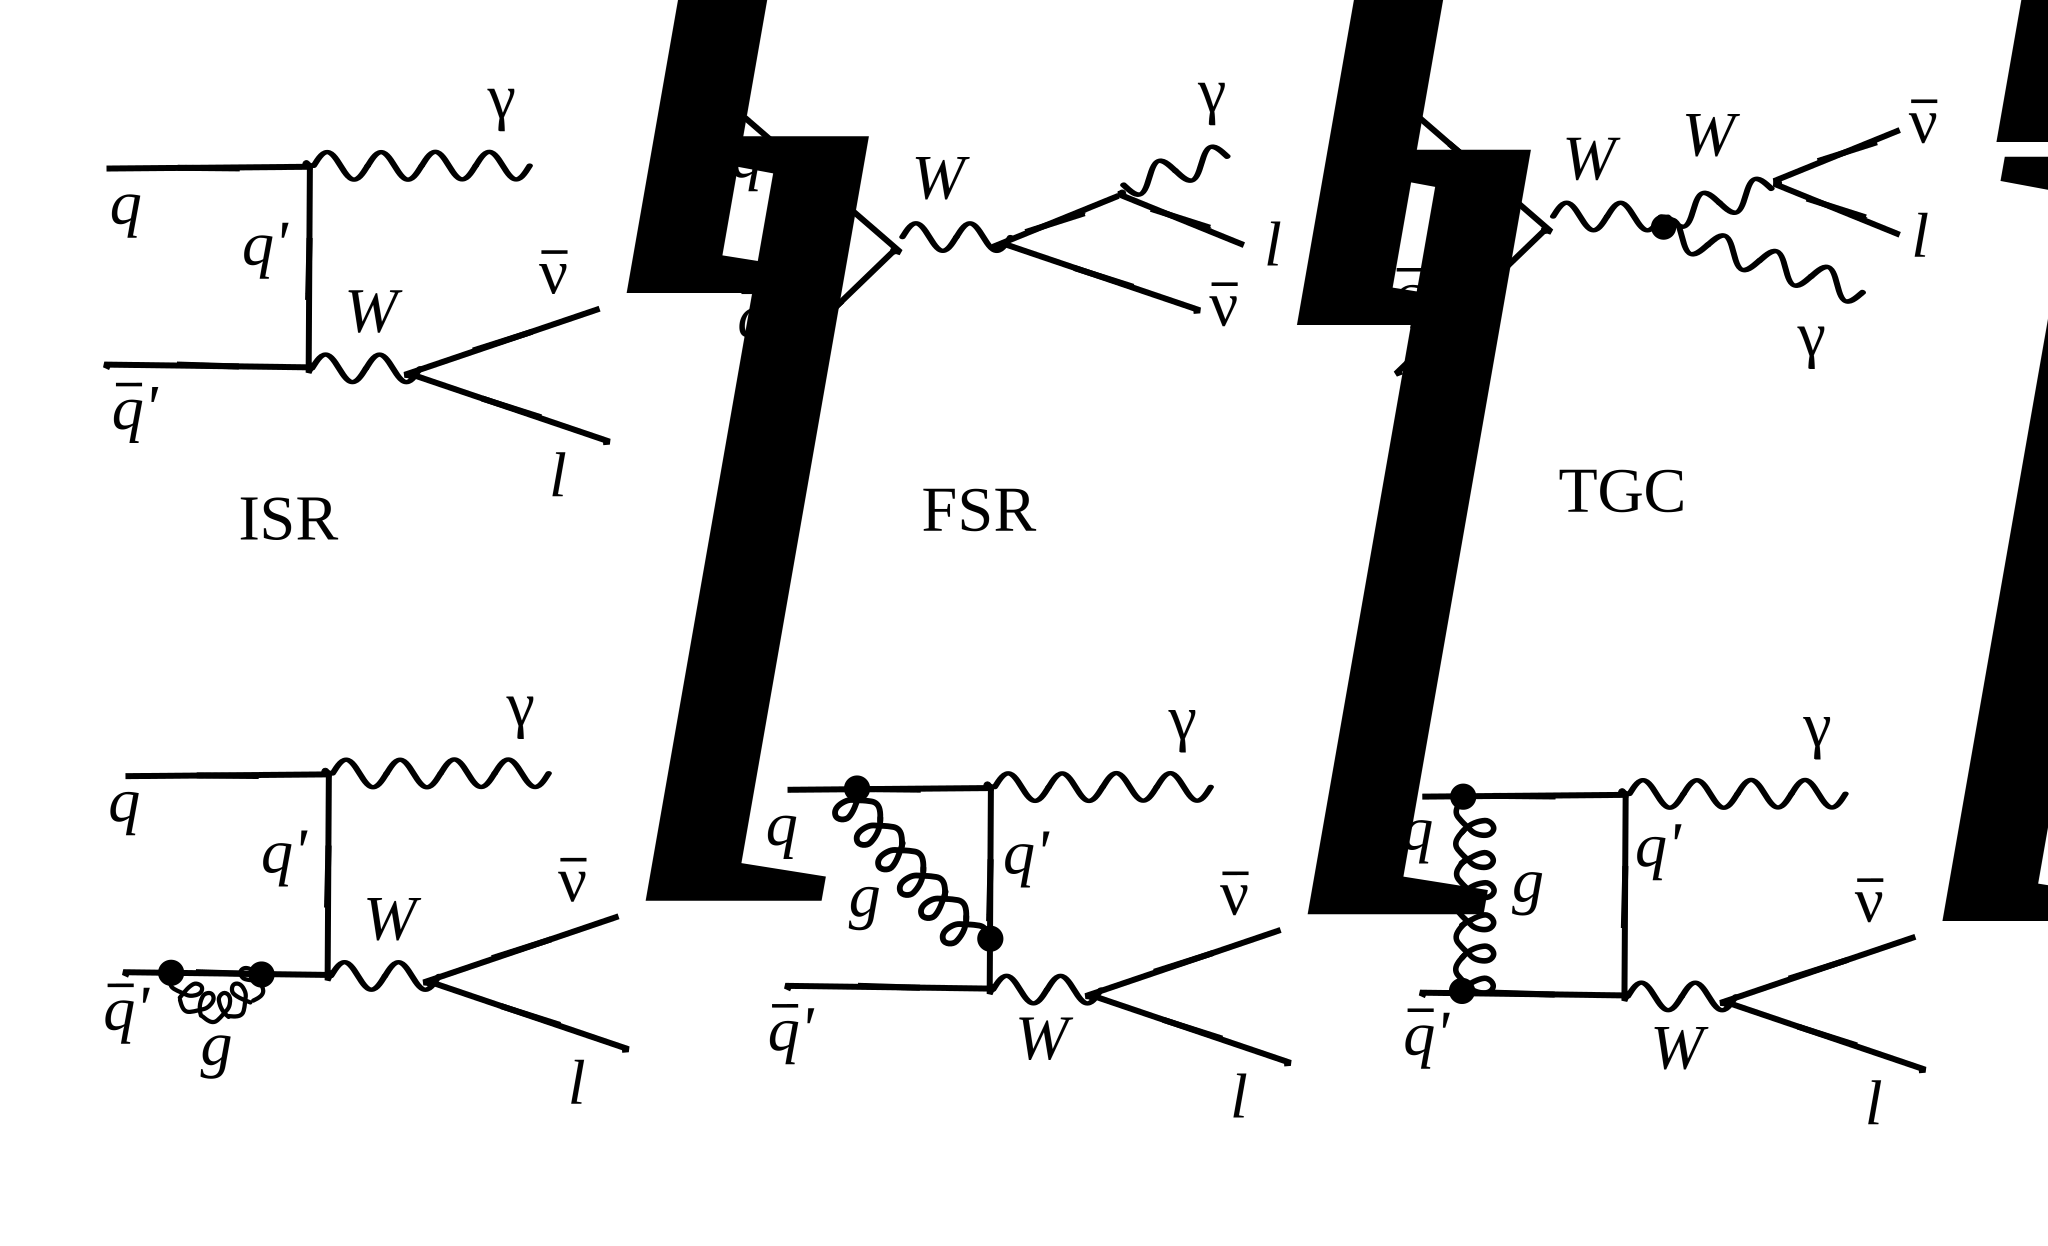
\includegraphics[width=0.90\textwidth]{../figs/WgAbout/feynmWg_LO_NLO.png}}
    % DRAW AND PLACE HERE A SCHEME OF THE CROSS SECTION FROM GRIFFITHS
    \caption{Illustration of the differential cross section concept in the classical case}
    \label{fig:CSclassical}
  \end{center}
\end{figure}

In this disseratation we are measuring the total and the differential cross section.\\

The cross section of an interaction of two particles can be interppreted as an area around one of the particles which has to be crossed by the other particles so that these two particles would interact. 
%REPHRASE PREVIOUS SENTENCE
The cross section characterizes the probability of two particles to interact. In the narrower case, the propability of two particles to interact in the exactly way to give a given final state.\\

A number of particles passing through the area $d\sigma$ per unit time is $dN=L \cdot d\sigma$, where L is the luminosity (the number of particles passing through the unit area per unit time). This expression is used to measure the cross section in collision experiments. The actual quantity which can be measured is a number of events of a given process and the luminosity is determined by collider characteristics. L may not be uniform in time however we are usually interested in measuring the total or differential cross section as a function of a certain kinematic paratemeter of a final state particle or of a system of final state particles.\\  
However, to measure the cross section we need to know total number of events of the given process but we cannot detect events which are out of the detector acceptance or which do not fall into the selection criteria we are using in the analysis. Therefore, the bnumber of events $dN$ has to be corrected in a measurement: $dN \rightarrow \frac{dN}{A \cdot \epsilon}$, where $A$ is a detector acceptance and $\epsilon$ is an efficiency of a signal process to pass selection conditions. Other corrections to $dN$ may have to be applied depending on the analysis.\\ 

To compute a cross section theoretically, one has to use Fermi's Golden rule which for the scattering of two particles\\
$1+2\rightarrow 3+4+...+n$\\
has the following form:\\

$\sigma = \frac{S \hbar^2 }{4\sqrt{(p_1p_2)^2-(m_1m_2c^2)^2}} \int |M|^2 (2\pi)^4 \delta^4(p_1+p_2-p_3-p_4-...-p_n) \prod_{j=3}^{n} \frac{1}{2 \sqrt{\bar{p_j^2}+m_j^2 c^2}}\frac{d^3\bar{p_j}}{(2\pi)^3} $\\

To estimate the amplitude $M$, one has to use the Feynman calculus. In Feynman calculus each vertex is assigned a vertex factor which include a coupling constant. For electromagnetic or weak interactions the coupling constant is always much less than one, for strong interactions the coupling constant depends on energy we are dealing with.  \\

In case of $W\gamma$, the cross section is the probability of a quark and an antiquark to annihilate with the production of a lepton ($\mu^{\pm}$ or $e^{\pm}$), a neutrino or antineutrino and a photon. Several of the corresponding Feynman diagrams are shown in Fig. \ref{fig:feynmWg_LO_NLO}. \\

The energy is high enough for coupling constant of the strong interactions to be less than one and, therefore, the Feynman diagrams with fewer vertices would give a significantly larger contribution to the amplitude. The perturbative theory can be used. The minimal number of vertices for the $W\gamma$ process is three which correspond to the diagrams in Fig. \ref{fig:feynmWg_LO_NLO}, top. The amplitudes from these diagrams form the leading order contribution to the cross section (LO).\\ 

There are many NLO corrections are possible to these diagrams. QED corrections would mean radiations of extra photons by charged particles, exchange of photons between different charged particles or a photon can be radiated and absorbed by the same charged particle forming a loop. Similarly, weak corrections are possible however they would be much weaker than the QED corrections. But even the QED corrections are too weak compared to QCD corrections which include gluon loops at the same quark line and exchange of a gluon between two different quark lines (Fig. \ref{fig:feynmWg_LO_NLO}, bottom).\\

%Provide theoretical cross section and order. FSR, ISR, TGC
%Need theory paper
